% Shared preamble for the English summaries in this repository.
\documentclass[11pt,a4paper]{article}
\usepackage[margin=2.2cm]{geometry}
\usepackage[T1]{fontenc}
\usepackage[utf8]{inputenc}
\usepackage{lmodern}
\usepackage{amsmath,amssymb}
\usepackage{graphicx}
\usepackage{booktabs}
\usepackage{enumitem}
\usepackage[hidelinks]{hyperref}
\setlist{itemsep=2pt,topsep=4pt}
\setlength{\parindent}{0pt}
\setlength{\parskip}{5pt}
\graphicspath{{figures/}}
\newcommand{\summaryheader}[3]{%
  \begin{center}
    {\Large\bfseries #2}\\[3pt]
    {\large #1}\\[3pt]
    {\small Arshia Goshtasbi \textbullet{} MSc Electrical Engineering (Control), Iran University of Science and Technology \textbullet{} #3}
  \end{center}
  \vspace{2pt}\hrule\vspace{8pt}\par}

\begin{document}
\summaryheader{Fuzzy Control, Project 2}{Fuzzy Speed Control of a DC Motor with Saturation, Dead Zone and Friction}{Autumn 1403 (2024)}

\textbf{Plant.} Armature current $i$ and speed $\omega$ follow
\[ L\dot i=f_{DZ}(V)-Ri-K_e(i)\,\omega,\qquad J\dot\omega=K_t(i)\,i-B\omega-\tau_c\,\mathrm{sign}(\omega)-T_L, \]
with magnetic saturation $K_{e,t}(i)=K_{e0,t0}\,i/\sqrt{i^2+I_s^2}$, an input dead zone of $V_{DZ}=2$\,V and $|V|\le24$\,V. Values: $R=1\,\Omega$, $L=0.5$\,H, $K_{e0}=K_{t0}=0.05$, $J=0.01$\,kg\,m$^2$, $B=0.003$\,N\,m\,s, $I_s=5$\,A, Coulomb friction $\tau_c=0.2$\,N\,m and load $T_L=0.2$\,N\,m ($0.3$ in the SMC case). The task is to track $\omega^\star=50$\,rad/s. All simulations use explicit Euler with $\Delta t=10^{-4}$\,s.

\textbf{Controllers} (one script each):
\begin{itemize}
  \item \texttt{Q\_OpenLoop}: $24$\,V applied; the motor settles near $120$\,rad/s, which shows the need for feedback.
  \item \texttt{Q\_PIDClassic}: PID with $K_p=10$, $K_i=2$, $K_d=2$, as a baseline.
  \item \texttt{Q\_Linear}: a fuzzy controller designed as for a linear plant. It has one input (the error), 31 triangular sets on $[-50,50]$, and a centre-average output on $[-240,240]$\,V before saturation, so it acts like a nonlinear proportional controller.
  \item \texttt{Q\_FuzzyPID}: a fuzzy supervisor tunes $K_p\in[1,10]$, $K_i\in[0,5]$ and $K_d\in[0,5]$ online from the error and its derivative (7 sets each, three $7\times7$ rule tables).
  \item \texttt{Q\_SMC\_Lambda}: sliding-mode control $V=K\,\mathrm{sat}(s/\phi)$ with $s=\lambda e+\dot e$, $K=20$ and $\phi=0.5$, where a 7-rule fuzzy system adapts the slope $\lambda\in[0.1,10]$.
\end{itemize}

\textbf{Results} (re-run in MATLAB R2023b; \texttt{tools/step\_metrics.m}):

\begin{center}\begin{tabular}{lrrrr}
\toprule
Controller & Rise 10--90\% (s) & Overshoot (\%) & Settling 2\% (s) & Final error (rad/s) \\
\midrule
Classic PID & 0.97 & 16.6 & 12.6 & $-0.22$ \\
Fuzzy, one input (10 s run) & 0.97 & 2.7 & not settled & 3.31 \\
Fuzzy-tuned PID & 0.97 & 37.9 & 7.3 & $0.00$ \\
SMC with fuzzy $\lambda$ & 1.95 & 0 & 3.3 & 0.12 \\
\bottomrule
\end{tabular}\end{center}

The single-input fuzzy controller has no integral action, so the load and friction leave a steady-state error. The fuzzy-tuned PID removes the error and settles faster than the fixed PID, but it overshoots more while the input is saturated at the start. Sliding-mode control with the fuzzy slope gives no overshoot and the shortest settling time; the boundary layer leaves a small error of $0.12$\,rad/s.

\begin{figure}[h]\centering
  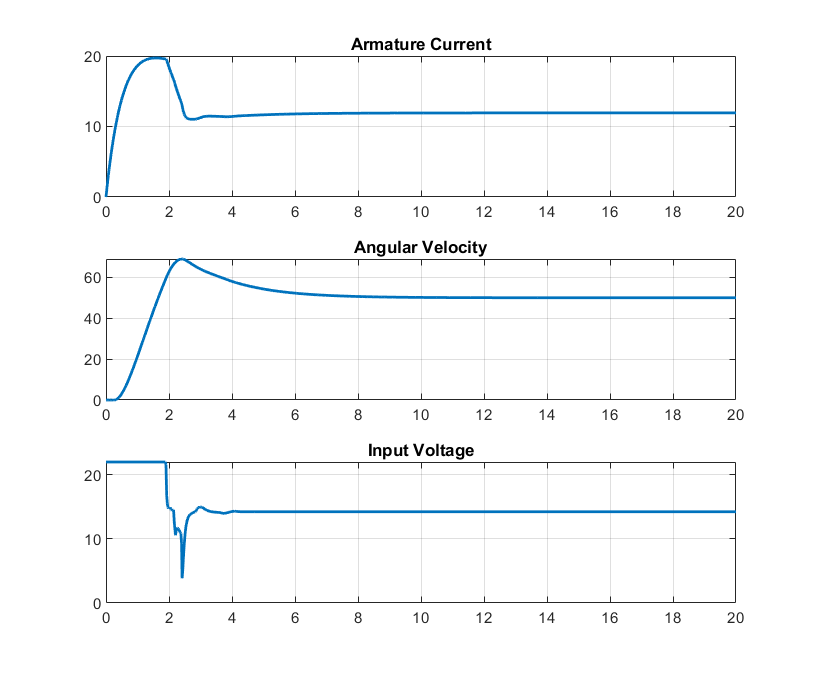
\includegraphics[width=.48\linewidth]{Q_FuzzyPID_1.png}\hfill
  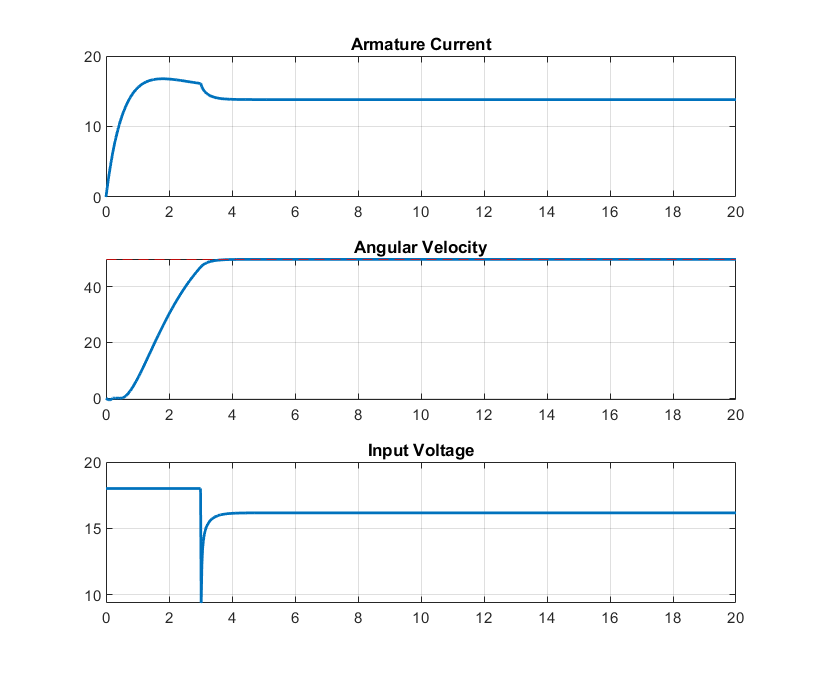
\includegraphics[width=.48\linewidth]{Q_SMC_Lambda_1.png}
  \caption{Current, speed and voltage with the fuzzy-tuned PID (left) and SMC with fuzzy $\lambda$ (right).}
\end{figure}
\end{document}
